\documentclass[a4paper,12pt]{article}
\usepackage{srs}  % Import the custom stylesheet

\begin{document}

% Title page
\SRSTitlePage{my songbook}{1.0}

% Table of Contents
\tableofcontents

\section{overview}
When playing in a band, you need to agree on a song structure (chords, breaks, bars, lyrics, ...). There are a lot of way to do that, you can have
partitions, use some free or commercial software ( lilypond, guitarpro, musescore, ... ). Each one has its pros and cons.

What we want here is to generate pdf files, that can be printed or viewed on a phone or tablet, and used during music practice, to communicate
between member of the bands. We want a synthetic view, where everything stands in one page (not the lyrics or the details)

\begin{figure}[h]  % h = here, t = top, b = bottom (placement options)
	\centering  % Centers the image
	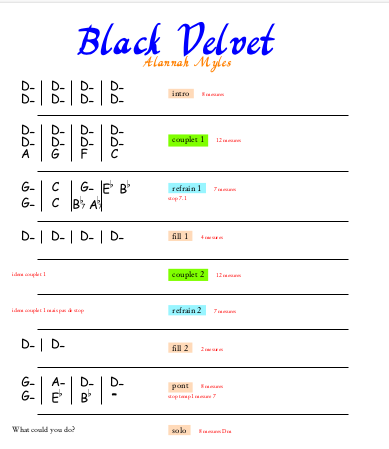
\includegraphics[width=0.5\textwidth]{doc1}  % Adjust the width as needed
	\caption{This is a sample image.}
	\label{fig:sample_image}  % Label for referencing the image
\end{figure}

\newpage

\req{the inputs are text files}

\req{each song of will be an independant input}


\req{a book is a list of songs}
It will be possible to define a book as a text file, and generate the output as one pdf file, this will contains all the songs.

\req{the outputs are pdf files}

\req{the outputs are pdf files}

\end{document}
